\documentclass{beamer}
\usetheme[height=7mm]{Rochester}
\usepackage{listings}
\usepackage{url}

%\usefonttheme{serif}

\usepackage[T1]{fontenc}
\usepackage{inconsolata}

\usepackage[absolute,overlay]{textpos} 
\newenvironment{reference}[2]{% 
  \begin{textblock*}{\textwidth}(#1,#2) 
      \tiny\bgroup\color{red!50!black}}{\egroup\end{textblock*}} 


\begin{document}

%%%%%%%%%%%%%%%%%%%%%%%%%%%%%%%%%%%%%%%%%%%%%%%%%%%%%%%%%%%%%%%%%%%%%%%%%%%%%%%%
%%%%%%%%%%%%%%%%%%%%%%%%%%%%%%%%%%%%%%%%%%%%%%%%%%%%%%%%%%%%%%%%%%%%%%%%%%%%%%%%
\title{Profile and reorder code execution in Geant4 to increase performance}
\subtitle{A Google Summer of Code Project}
\author{Stathis Kamperis}
\institute{
  Department of Physics\\
  Aristotle University of Thessaloniki\\
  Greece\\[1ex]
  \texttt{ekamperi@gmail.com}
}
\date{August, 2012}

%%%%%%%%%%%%%%%%%%%%%%%%%%%%%%%%%%%%%%%%%%%%%%%%%%%%%%%%%%%%%%%%%%%%%%%%%%%%%%%%
%%%%%%%%%%%%%%%%%%%%%%%%%%%%%%%%%%%%%%%%%%%%%%%%%%%%%%%%%%%%%%%%%%%%%%%%%%%%%%%%
\begin{frame}[plain]
  \titlepage
\begin{reference}{4mm}{85mm}
version: 256@89329
\end{reference} 
\end{frame}

%%%%%%%%%%%%%%%%%%%%%%%%%%%%%%%%%%%%%%%%%%%%%%%%%%%%%%%%%%%%%%%%%%%%%%%%%%%%%%%%
%%%%%%%%%%%%%%%%%%%%%%%%%%%%%%%%%%%%%%%%%%%%%%%%%%%%%%%%%%%%%%%%%%%%%%%%%%%%%%%%
\begin{frame}{Overview}

Geant4
\begin{itemize}
  \item Large source code base
  \item Lots of classes
  \item Highly conditionalized code
  \item Complex numerical calculations
\end{itemize}

Full CMS
\begin{itemize}
	\item Complex geometry and physics
\end{itemize}

\begin{center}
	\fcolorbox{red}{white}{Very low visibility to the runtime aspects of the simulations}
\end{center}
\end{frame}

%%%%%%%%%%%%%%%%%%%%%%%%%%%%%%%%%%%%%%%%%%%%%%%%%%%%%%%%%%%%%%%%%%%%%%%%%%%%%%%%
%%%%%%%%%%%%%%%%%%%%%%%%%%%%%%%%%%%%%%%%%%%%%%%%%%%%%%%%%%%%%%%%%%%%%%%%%%%%%%%%
\begin{frame}{Profiling targets}

\begin{itemize}
	\item Full CMS experiment
	\item Simplified Calorimeter

	\begin{itemize}
		\item Faster initialization, faster profiling cycles
		\item Simpler Geometry
		\begin{itemize}
			\item Useful for examining how (lack of complex) geometry affects performance
		\end{itemize}
	\end{itemize}
	
\item Examples bundled with Geant4
	
\end{itemize}
\end{frame}

%%%%%%%%%%%%%%%%%%%%%%%%%%%%%%%%%%%%%%%%%%%%%%%%%%%%%%%%%%%%%%%%%%%%%%%%%%%%%%%%
%%%%%%%%%%%%%%%%%%%%%%%%%%%%%%%%%%%%%%%%%%%%%%%%%%%%%%%%%%%%%%%%%%%%%%%%%%%%%%%%
\begin{frame}{Profiling tools}

\textcolor{blue}{Ported Geant4 to Solaris 11/x64}

\begin{itemize}
	\item DTrace

	\begin{itemize}
		\item A dynamic tracing framework
		\item Available also in Mac OSX (an officially supported platform by Geant4)
		\item Fine-grained profiling
	\end{itemize}

	\item mdb (Modular debugger)

	\item cputrack
	\begin{itemize}
		\item Access CPU performance counters
		\item data cache misses, instruction cache misses, branch mispredictions, ...
	\end{itemize}
\end{itemize}	

\end{frame}

%%%%%%%%%%%%%%%%%%%%%%%%%%%%%%%%%%%%%%%%%%%%%%%%%%%%%%%%%%%%%%%%%%%%%%%%%%%%%%%%
%%%%%%%%%%%%%%%%%%%%%%%%%%%%%%%%%%%%%%%%%%%%%%%%%%%%%%%%%%%%%%%%%%%%%%%%%%%%%%%%
\begin{frame}{Profiling tools - cont.}

\begin{itemize}
	\item libumem
	
	\begin{itemize}
		\item Useful for debugging memory problems (leaks, corruptions, etc)
		\item As simple as running: LD\_PRELOAD=libumem.so.1 ./a.out
		\item Can be used in conjuction with mdb \(::findleaks, ::umem\_verify, ...\)
	\end{itemize}
	
	\item pbind (to bind profiled process to a specific CPU)
	\item A pseudo device driver to invalidate CPU caches on demand
	\item Visualisation tools and Statistics
	
	\begin{itemize}
		\item gnuplot, ggplot2, R
	\end{itemize}
\end{itemize}
\end{frame}

%%%%%%%%%%%%%%%%%%%%%%%%%%%%%%%%%%%%%%%%%%%%%%%%%%%%%%%%%%%%%%%%%%%%%%%%%%%%%%%%
%%%%%%%%%%%%%%%%%%%%%%%%%%%%%%%%%%%%%%%%%%%%%%%%%%%%%%%%%%%%%%%%%%%%%%%%%%%%%%%%
\begin{frame}{Profiling tools - Alternatives}

\textcolor{blue}{Not propagandizing in favor of Solaris}

\vspace{5mm}

Alternatives for Linux users:

\begin{itemize}
	\item DTrace $\rightarrow$ SystemTap
	\item mdb $\rightarrow$ gdb
	\item cputrack $\rightarrow$ perf, cachegrind
	\item libumem $\rightarrow$ valgrind
	\item pbind $\rightarrow$ taskset
\end{itemize}

The rest are common for both platforms (visualisation and statistics)

\end{frame}

%%%%%%%%%%%%%%%%%%%%%%%%%%%%%%%%%%%%%%%%%%%%%%%%%%%%%%%%%%%%%%%%%%%%%%%%%%%%%%%%
%%%%%%%%%%%%%%%%%%%%%%%%%%%%%%%%%%%%%%%%%%%%%%%%%%%%%%%%%%%%%%%%%%%%%%%%%%%%%%%%
\begin{frame}{DTrace}

\begin{itemize}
\item pid provider
\item Flamegraphs
\item USDT (user-level statically defined tracing)
\item Speculative tracing
\item All of the above combined
\end{itemize}
\end{frame}


%%%%%%%%%%%%%%%%%%%%%%%%%%%%%%%%%%%%%%%%%%%%%%%%%%%%%%%%%%%%%%%%%%%%%%%%%%%%%%%%
%%%%%%%%%%%%%%%%%%%%%%%%%%%%%%%%%%%%%%%%%%%%%%%%%%%%%%%%%%%%%%%%%%%%%%%%%%%%%%%%
\begin{frame}{DTrace - pid provider}
\begin{reference}{4mm}{85mm}
It allows to trace arbitrary instructions inside a function, as it will be
demonstrated later.
\end{reference} 

\textcolor{blue}{Definition} pid provider allows for tracing of the entry and
return of any function in a user process

\vspace{5mm}

The pid provider has no probe effect when probes are not enabled.
\end{frame}


%%%%%%%%%%%%%%%%%%%%%%%%%%%%%%%%%%%%%%%%%%%%%%%%%%%%%%%%%%%%%%%%%%%%%%%%%%%%%%%%
%%%%%%%%%%%%%%%%%%%%%%%%%%%%%%%%%%%%%%%%%%%%%%%%%%%%%%%%%%%%%%%%%%%%%%%%%%%%%%%%

\begin{frame}[fragile]{DTrace - pid provider 1}
\textcolor{blue}{How many times does the {\tt G4Allocator} grow in size during 100 simulated events ?}

\lstset{frame=single, columns=flexible}
\lstset{basicstyle=\tiny\ttfamily}
\begin{lstlisting}
# dtrace -n '
pid$target::*G4AllocatorPool*Grow*:entry
{
    @ = count();
}' -c '/home/stathis/geant4.9.5.p01/bin/full_cms ./bench1_100.g4'

             5921
\end{lstlisting}

\textcolor{blue}{How much time do the above resizes consume ?}

\lstset{frame=single, columns=flexible}
\lstset{basicstyle=\tiny\ttfamily}
\begin{lstlisting}
dtrace -n '
pid$target::*G4AllocatorPool*Grow*:entry
{
    self->ts = vtimestamp;
}

pid$target::*G4AllocatorPool*Grow*:return
/self->ts/
{
    @ = sum((vtimestamp - self->ts)/1000);
    self->ts = 0;
}' -c '/home/stathis/geant4.9.5.p01/bin/full_cms ./bench1_100.g4'
             4859  # ~5 msec
\end{lstlisting}
\end{frame}

%%%%%%%%%%%%%%%%%%%%%%%%%%%%%%%%%%%%%%%%%%%%%%%%%%%%%%%%%%%%%%%%%%%%%%%%%%%%%%%%
%%%%%%%%%%%%%%%%%%%%%%%%%%%%%%%%%%%%%%%%%%%%%%%%%%%%%%%%%%%%%%%%%%%%%%%%%%%%%%%%
\begin{frame}[fragile]{DTrace - pid provider 2}
\textcolor{blue}{How do we skip the initialization part of Geant4/Full CMS ?}
\begin{itemize}
\item Use a predicate that checks whether we are inside the DoEventLoop()
\end{itemize}

\lstset{frame=single, columns=flexible}
\lstset{basicstyle=\tiny\ttfamily}
\begin{lstlisting}
dtrace -n '
BEGIN
{
    tracing = 0;
}

pid$target::*DoEventLoop*:entry  { tracing = 1; }
pid$target::*DoEventLoop*:return { exit(0);     }

someprobe
/tracing != 0/
{
    ...
}
' -c '/home/stathis/geant4.9.5.p01/bin/full_cms ./bench_100.g4'
\end{lstlisting}

\end{frame}

%%%%%%%%%%%%%%%%%%%%%%%%%%%%%%%%%%%%%%%%%%%%%%%%%%%%%%%%%%%%%%%%%%%%%%%%%%%%%%%%
%%%%%%%%%%%%%%%%%%%%%%%%%%%%%%%%%%%%%%%%%%%%%%%%%%%%%%%%%%%%%%%%%%%%%%%%%%%%%%%%
\begin{frame}{USDT (user-level statically defined tracing)}

{\bf \textcolor{blue}{Allows to place custom probe points in application code}}

\begin{itemize}
	\item Available {\bf both} in development and production builds
	
	\begin{itemize}
		\item No need to recompile with a debug flag set
	\end{itemize}
	
	\item DTrace dynamically activates the probes when asked
	
	\begin{itemize}
		\item By {\bf dynamically} rewriting the instructions of the profiled app
	\end{itemize}

	\item {\bf Negligible overhead} when not in use (a few NOPs)
	
	\item Take advantage of DTrace {\bf rich reporting capabilities (aggregations)}
\end{itemize}

\end{frame}

%%%%%%%%%%%%%%%%%%%%%%%%%%%%%%%%%%%%%%%%%%%%%%%%%%%%%%%%%%%%%%%%%%%%%%%%%%%%%%%%
%%%%%%%%%%%%%%%%%%%%%%%%%%%%%%%%%%%%%%%%%%%%%%%%%%%%%%%%%%%%%%%%%%%%%%%%%%%%%%%%
\begin{frame}{USDT (user-level statically defined tracing)}
\begin{itemize}
\item \textcolor{blue}{simple\_provider.d}: defines the provider probes and argument-
linked into the module binary at link time
\item \textcolor{blue}{simple\_provider.h}: defines the structure passed from Geant4
to DTrace at run time
\item \textcolor{blue}{G4SmartTrackStack.cc}: uses hooks at the end of each push pop operation
to fire the corresponding DTrace probes
\end{itemize}
\end{frame}

%%%%%%%%%%%%%%%%%%%%%%%%%%%%%%%%%%%%%%%%%%%%%%%%%%%%%%%%%%%%%%%%%%%%%%%%%%%%%%%%
%%%%%%%%%%%%%%%%%%%%%%%%%%%%%%%%%%%%%%%%%%%%%%%%%%%%%%%%%%%%%%%%%%%%%%%%%%%%%%%%
\begin{frame}[fragile]{USDT - Example 1}
\lstset{basicstyle=\tiny\ttfamily}

\textcolor{blue}{Objective} Everytime we \textit{push} a track to the track manager or we \textit{pop} one from it,
dump the sizes of all stacks.

\lstset{frame=single, columns=flexible}
\begin{lstlisting}
# dtrace -qn '
simple$target:::
{
    printf("%s track=%d size=%d\n", probefunc, arg0, arg1);
}'
-c '/home/stathis/geant4.9.5.p01/bin/mainStatAccepTest ./exercise.g4' | c++filt -np
...
G4SmartTrackStack::PushToStack track=0 size=1
G4SmartTrackStack::PopFromStack track=0 size=0
G4SmartTrackStack::PushToStack track=2 size=1
G4SmartTrackStack::PushToStack track=2 size=2
G4SmartTrackStack::PushToStack track=2 size=3
G4SmartTrackStack::PushToStack track=0 size=1
...
G4SmartTrackStack::PopFromStack track=2 size=446
G4SmartTrackStack::PopFromStack track=2 size=445
G4SmartTrackStack::PopFromStack track=2 size=444
G4SmartTrackStack::PopFromStack track=2 size=443
\end{lstlisting}
\end{frame}

%%%%%%%%%%%%%%%%%%%%%%%%%%%%%%%%%%%%%%%%%%%%%%%%%%%%%%%%%%%%%%%%%%%%%%%%%%%%%%%%
%%%%%%%%%%%%%%%%%%%%%%%%%%%%%%%%%%%%%%%%%%%%%%%%%%%%%%%%%%%%%%%%%%%%%%%%%%%%%%%%
\begin{frame}[fragile]{USDT - Example 2}
\lstset{basicstyle=\tiny\ttfamily}

\textcolor{blue}{Objective} Print the distribution of stack sizes for unclassified particles
(primaries + any particle not beloning to the set ${n^0, e^-,\gamma, e^+}$

\lstset{frame=single, columns=flexible}
\begin{lstlisting}
# dtrace -qn '
simple$target:::
/arg0==1/
{
    @["distribution of 1st stack's size"] = quantize(arg1);
}' -c '/home/stathis/geant4.9.5.p01/bin/mainStatAccepTest ./exercise.g4'
^C
  distribution of 1st stack's size
           value  ------------- Distribution ------------- count
              -1 |                                         0
               0 |                                         111
               1 |                                         308
               2 |@                                        963
               4 |@                                        2241
               8 |@@                                       3193
              16 |@@@                                      4452
              32 |@@@@@                                    7700
              64 |@@@@@@@@@@                               15574
             128 |@@@@@@@@@@@@@@@                          23497
             256 |@@@                                      4459
             512 |                                         0
\end{lstlisting}
\end{frame}

%%%%%%%%%%%%%%%%%%%%%%%%%%%%%%%%%%%%%%%%%%%%%%%%%%%%%%%%%%%%%%%%%%%%%%%%%%%%%%%%
%%%%%%%%%%%%%%%%%%%%%%%%%%%%%%%%%%%%%%%%%%%%%%%%%%%%%%%%%%%%%%%%%%%%%%%%%%%%%%%%
\begin{frame}{USDT - Example 3}

\textcolor{blue}{Objective} Visualize the size of stacks and the total energy of their particles

\vspace{1mm}

The following graph is from a simulation of 2 events in Full CMS:

\begin{center}
  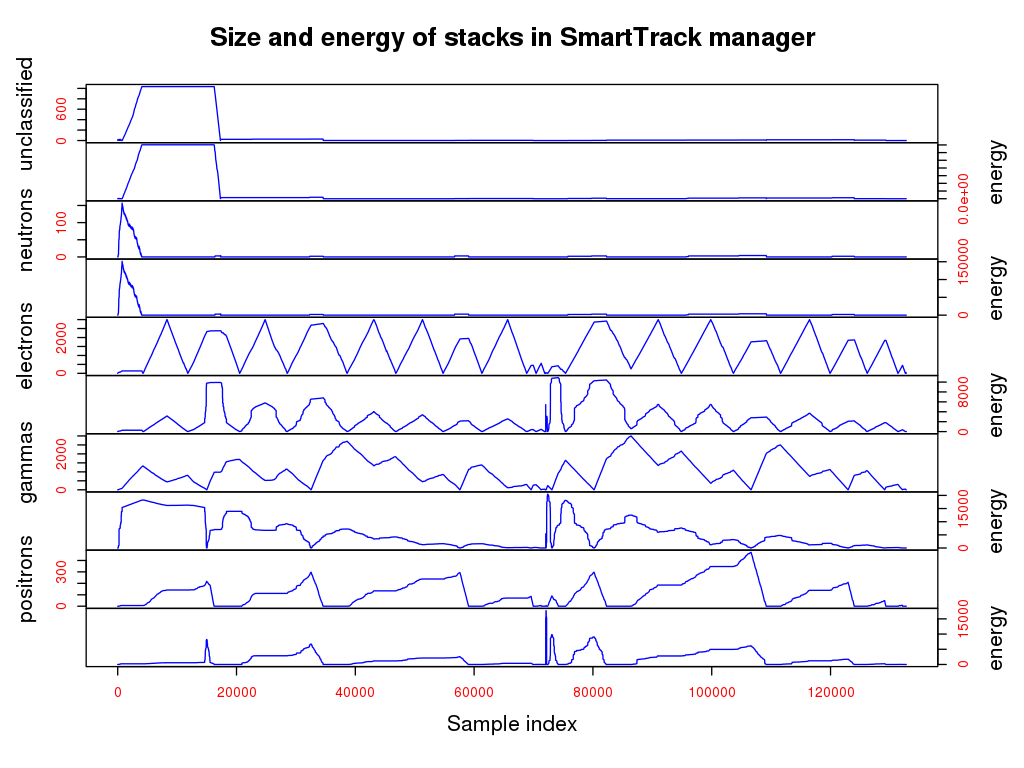
\includegraphics[width=0.8\textwidth]{smarttracksize-ts-2evts-energy.png}
\end{center}
\end{frame}

%%%%%%%%%%%%%%%%%%%%%%%%%%%%%%%%%%%%%%%%%%%%%%%%%%%%%%%%%%%%%%%%%%%%%%%%%%%%%%%%
%%%%%%%%%%%%%%%%%%%%%%%%%%%%%%%%%%%%%%%%%%%%%%%%%%%%%%%%%%%%%%%%%%%%%%%%%%%%%%%%
\begin{frame}{Speculative tracing - Introduction}
\begin{reference}{4mm}{85mm}
From DTrace guide
\end{reference} 
\textcolor{blue}{Definition} The ability to tentatively trace data and then later decide whether to commit
the data to a tracing buffer or discard it.
\end{frame}

%%%%%%%%%%%%%%%%%%%%%%%%%%%%%%%%%%%%%%%%%%%%%%%%%%%%%%%%%%%%%%%%%%%%%%%%%%%%%%%%
%%%%%%%%%%%%%%%%%%%%%%%%%%%%%%%%%%%%%%%%%%%%%%%%%%%%%%%%%%%%%%%%%%%%%%%%%%%%%%%%
\begin{frame}{Speculative tracing - A real use case}

\textcolor{blue}{Problem} Some {\tt ProcessOneEvent()} need much more than
average time to complete

\begin{center}
  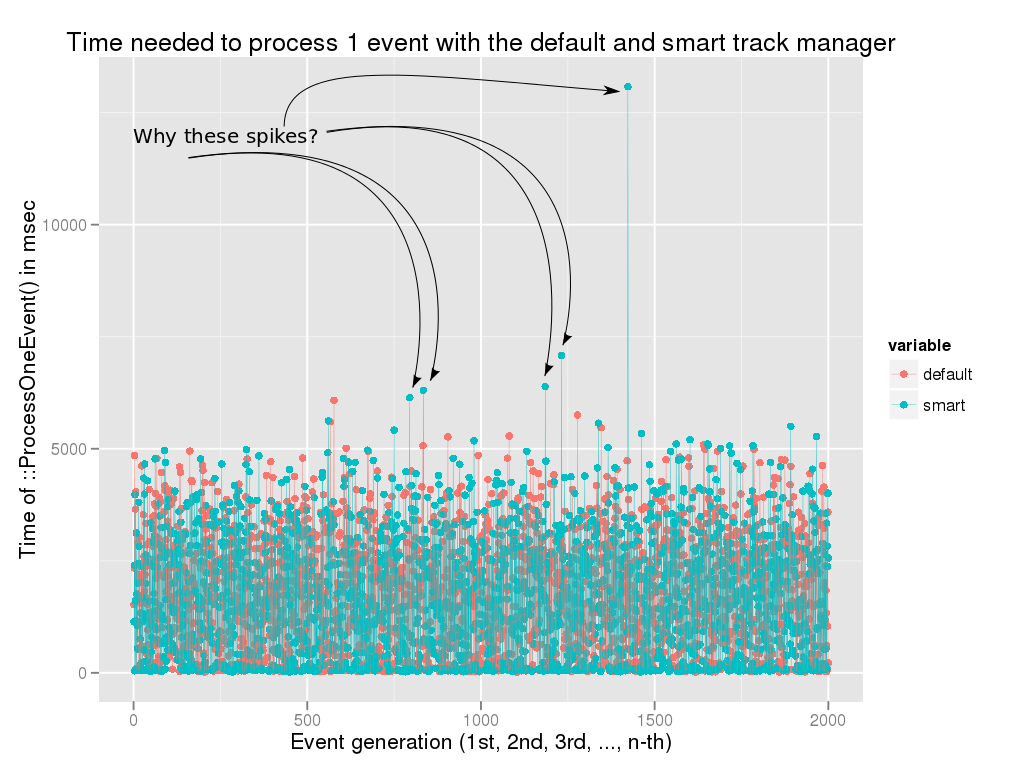
\includegraphics[width=0.8\textwidth]{evts1-arrows.png}
\end{center}
\end{frame}

%%%%%%%%%%%%%%%%%%%%%%%%%%%%%%%%%%%%%%%%%%%%%%%%%%%%%%%%%%%%%%%%%%%%%%%%%%%%%%%%
%%%%%%%%%%%%%%%%%%%%%%%%%%%%%%%%%%%%%%%%%%%%%%%%%%%%%%%%%%%%%%%%%%%%%%%%%%%%%%%%
\begin{frame}{Speculative tracing - A real use case}
\textcolor{blue}{Strategy} We are going to trace all {\tt ProcessOneEvent()} calls, but commit to our tracing
buffer \textit{only} those that behave bad.

\vspace{5mm}

In this context, "trace" refers to looking at stacks' sizes when {\tt ProcessOneEvent()}
stalls while processing the event.

\end{frame}

%%%%%%%%%%%%%%%%%%%%%%%%%%%%%%%%%%%%%%%%%%%%%%%%%%%%%%%%%%%%%%%%%%%%%%%%%%%%%%%%
%%%%%%%%%%%%%%%%%%%%%%%%%%%%%%%%%%%%%%%%%%%%%%%%%%%%%%%%%%%%%%%%%%%%%%%%%%%%%%%%
\begin{frame}[fragile]{Speculative tracing - A real use case cont.}
\lstset{basicstyle=\tiny\ttfamily}
\lstset{frame=single, columns=flexible}
\begin{lstlisting}
pid$target::*G4EventManager*ProcessOneEventEP7G4Event:entry
{
    self->pstart = vtimestamp;
    spec = speculation();
}

simple$target:::
/tracing && spec/
{
    speculate(spec);
    printf("%d %d %d %d %d\n", arg0, arg1, arg2, arg3, arg4);
}

pid$target::-:'$retaddr'
/self->pstart/
{
    self->t = (vtimestamp - self->pstart)/1000000;
    self->pstart = 0;
}

pid$target::-:'$retaddr'
/spec && self->t >= 4500/
{
    commit(spec);
    spec = 0;
}

pid$target::-:'$retaddr'
/spec && self->t < 4500/
{
    discard(spec);
    spec = 0;
}
\end{lstlisting}
\end{frame}

%%%%%%%%%%%%%%%%%%%%%%%%%%%%%%%%%%%%%%%%%%%%%%%%%%%%%%%%%%%%%%%%%%%%%%%%%%%%%%%%
%%%%%%%%%%%%%%%%%%%%%%%%%%%%%%%%%%%%%%%%%%%%%%%%%%%%%%%%%%%%%%%%%%%%%%%%%%%%%%%%
\begin{frame}{Speculative tracing - A real use case cont.}

\textcolor{blue}{Hint} The maximum desired size for all stacks was requested to be 400.

$e^-$ and $\gamma$ too often will not honour that limit.

\begin{center}
  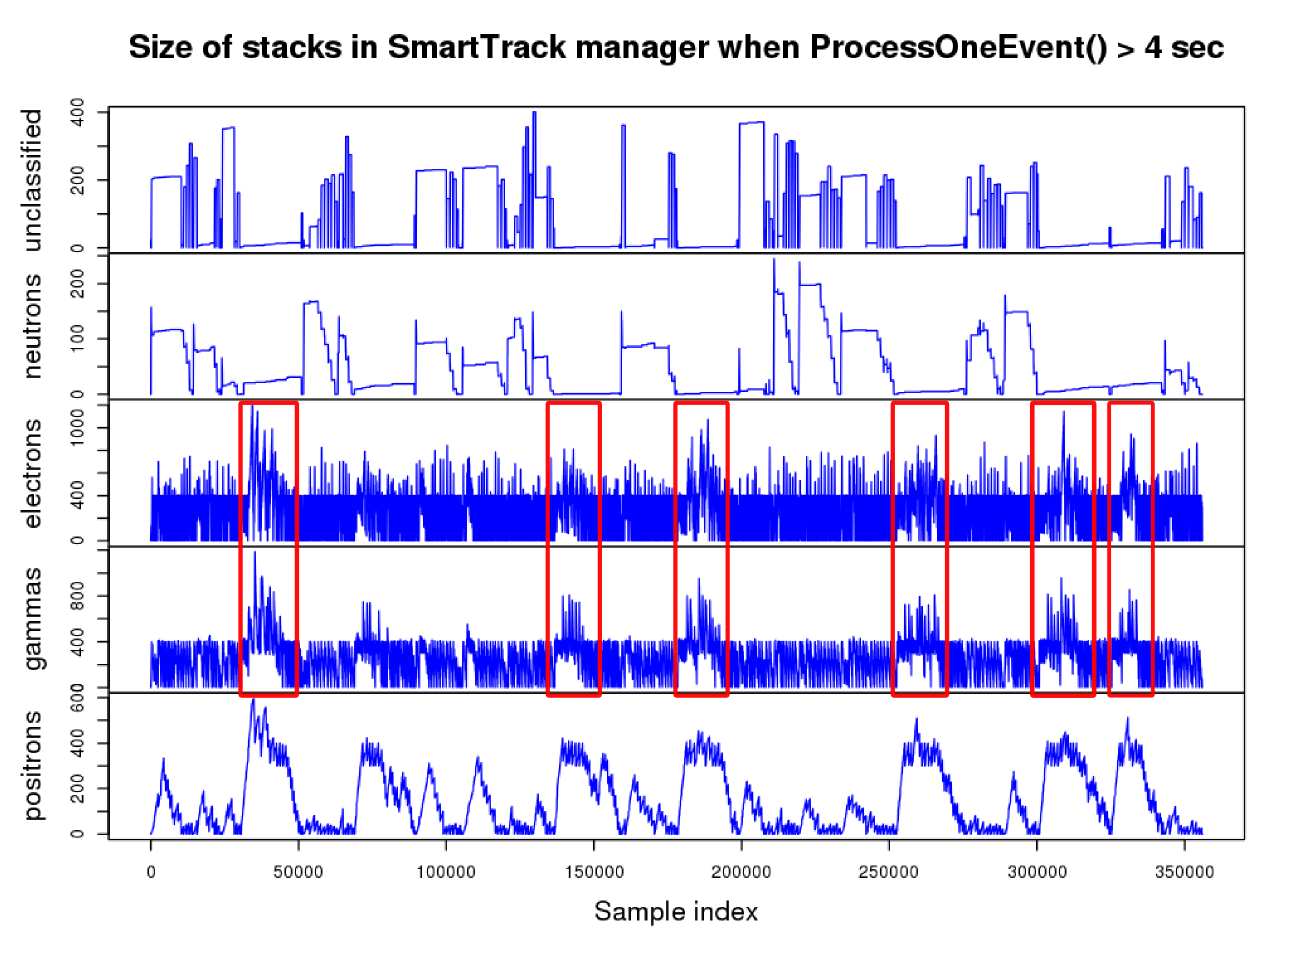
\includegraphics[width=0.8\textwidth]{pathol-all.png}
\end{center}
\end{frame}

%%%%%%%%%%%%%%%%%%%%%%%%%%%%%%%%%%%%%%%%%%%%%%%%%%%%%%%%%%%%%%%%%%%%%%%%%%%%%%%%
%%%%%%%%%%%%%%%%%%%%%%%%%%%%%%%%%%%%%%%%%%%%%%%%%%%%%%%%%%%%%%%%%%%%%%%%%%%%%%%%
\begin{frame}{Speculative tracing - A real use case cont. - Zoom 1/2}

\begin{center}
  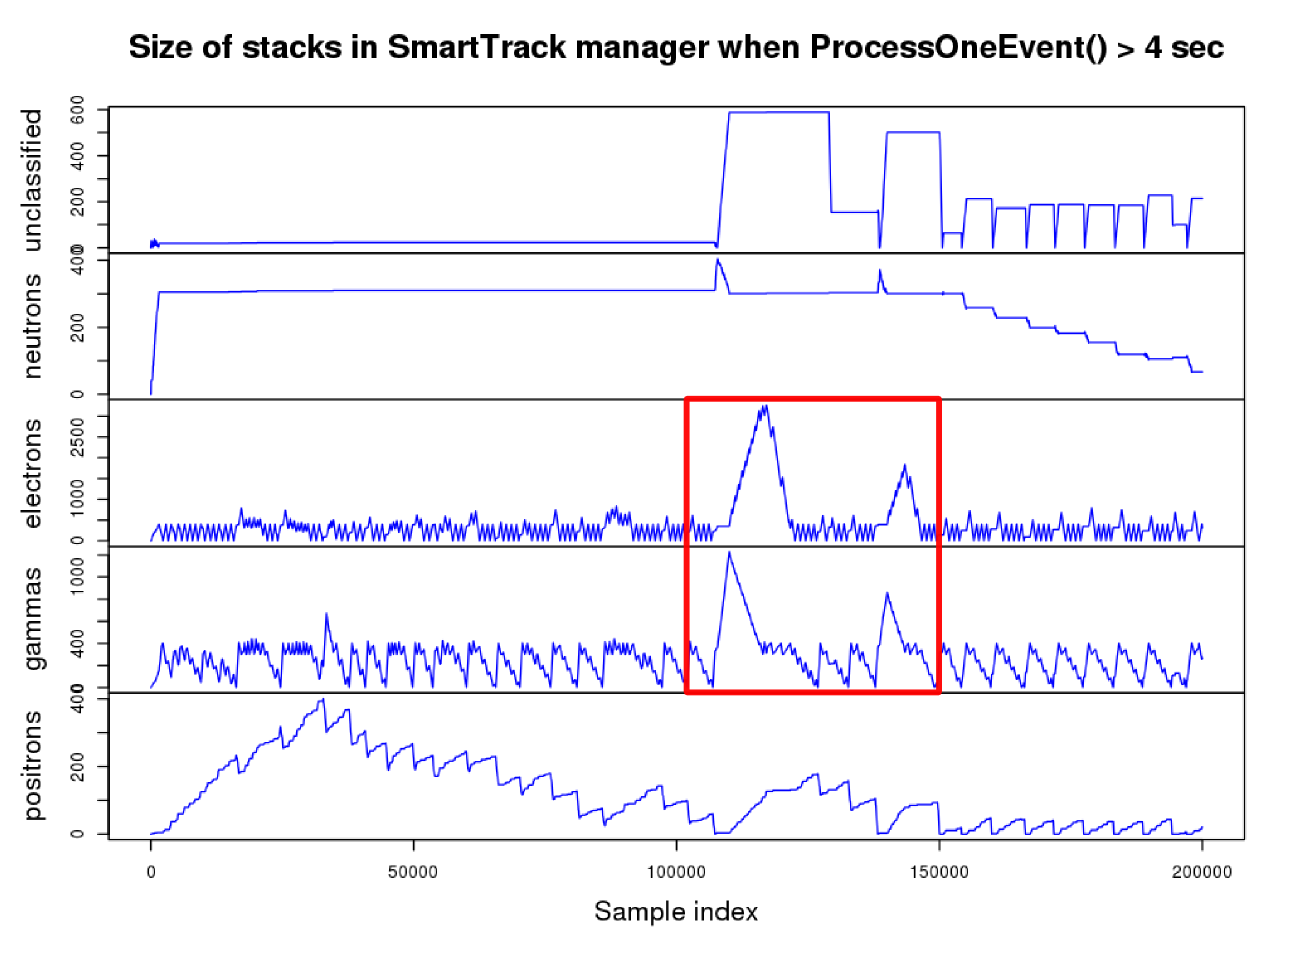
\includegraphics[width=0.8\textwidth]{pathol-zoom1.png}
\end{center}
\end{frame}

%%%%%%%%%%%%%%%%%%%%%%%%%%%%%%%%%%%%%%%%%%%%%%%%%%%%%%%%%%%%%%%%%%%%%%%%%%%%%%%%
%%%%%%%%%%%%%%%%%%%%%%%%%%%%%%%%%%%%%%%%%%%%%%%%%%%%%%%%%%%%%%%%%%%%%%%%%%%%%%%%
\begin{frame}{Speculative tracing - A real use case cont. - Zoom 2/2}

\begin{center}
  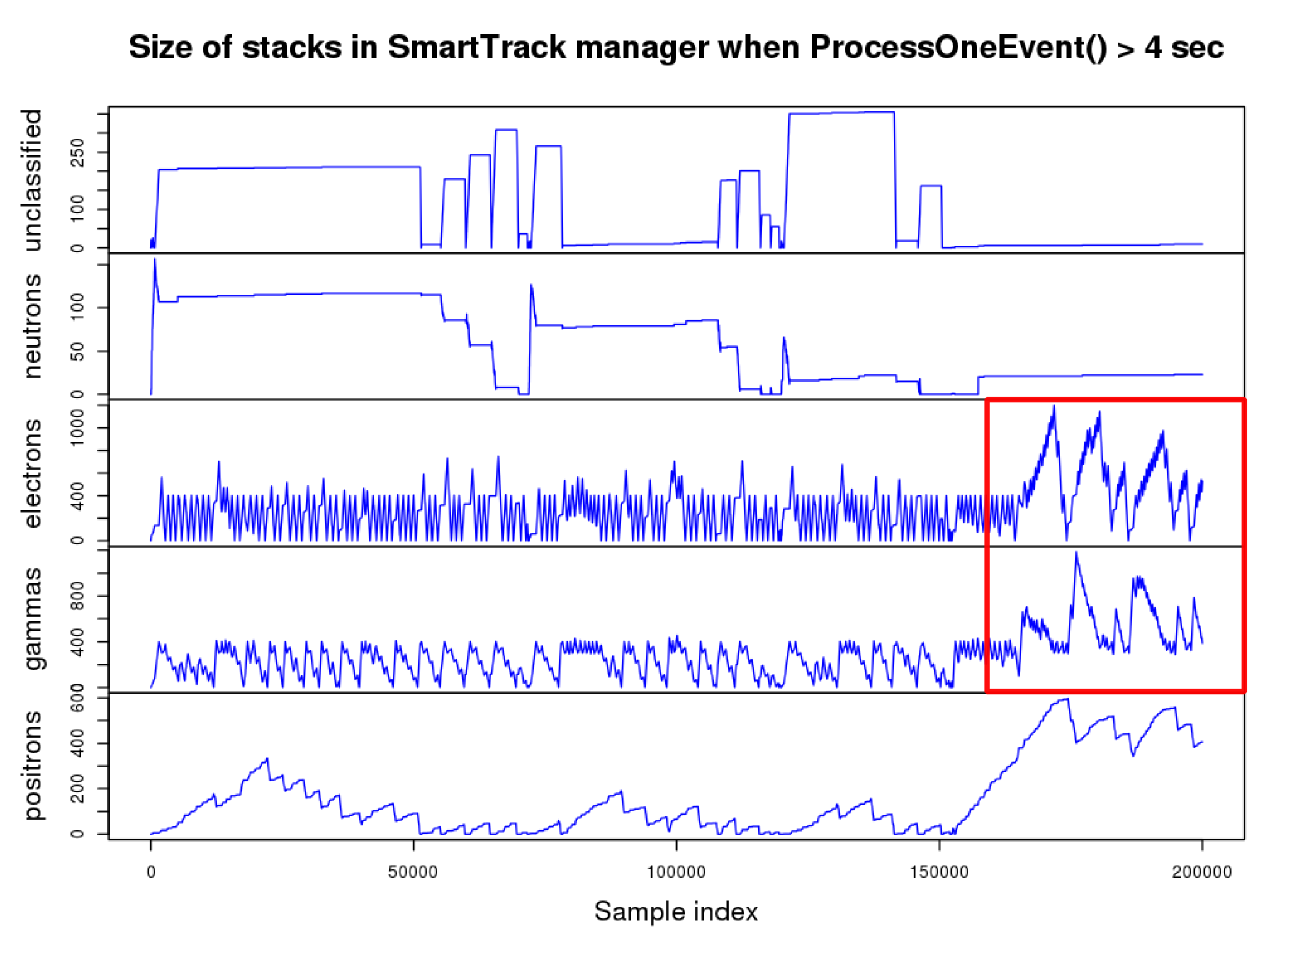
\includegraphics[width=0.8\textwidth]{pathol-zoom2.png}
\end{center}
\end{frame}

%%%%%%%%%%%%%%%%%%%%%%%%%%%%%%%%%%%%%%%%%%%%%%%%%%%%%%%%%%%%%%%%%%%%%%%%%%%%%%%%
%%%%%%%%%%%%%%%%%%%%%%%%%%%%%%%%%%%%%%%%%%%%%%%%%%%%%%%%%%%%%%%%%%%%%%%%%%%%%%%%
\begin{frame}{Flame graphs}
\textcolor{blue}{Definition} Flame graphs are a visualization method for sampled stack traces

\begin{center}
  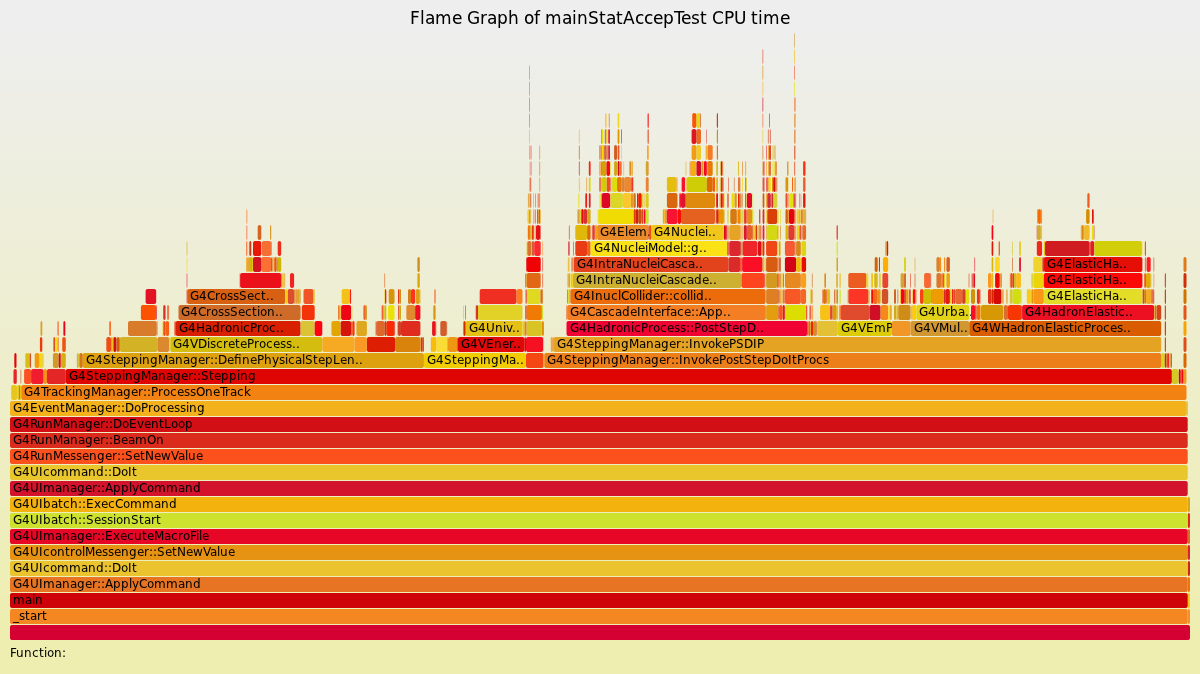
\includegraphics[width=1.0\textwidth]{timeflame.png}
\end{center}
\end{frame}

%%%%%%%%%%%%%%%%%%%%%%%%%%%%%%%%%%%%%%%%%%%%%%%%%%%%%%%%%%%%%%%%%%%%%%%%%%%%%%%%
%%%%%%%%%%%%%%%%%%%%%%%%%%%%%%%%%%%%%%%%%%%%%%%%%%%%%%%%%%%%%%%%%%%%%%%%%%%%%%%%
\begin{frame}{Flame graphs}
\textcolor{blue}{Scope} Anything that can be sampled by DTrace can be visualized as a flame graph

\begin{itemize}
	\item Function execution time
	\item Data cache misses
	\item Instruction cache misses
	\item Branch mispredictions
	\item Memory allocation sizes
	\item ...
\end{itemize}

\begin{reference}{4mm}{85mm}
	Developed by Brendan Gregg
\end{reference}
\end{frame}

\begin{frame}{Flame graphs}
\textcolor{blue}{Hints}

\begin{itemize}
	\item Identification of hot code-paths
	\item The x-axis is the sample population
	\item The y-axis is the stack depth
	\item The width of a box is proportional to the measured quantity. E.g.,
	\begin{itemize}
		\item A wide box means that a function either takes a lot of time to complete or
		that it is called too often (in either case the probability that its stack trace
		is sampled increases)
	\end{itemize}
	\item The colors are \textit{not} significant (they are picked at random to be "warm")
\end{itemize}
\end{frame}

%%%%%%%%%%%%%%%%%%%%%%%%%%%%%%%%%%%%%%%%%%%%%%%%%%%%%%%%%%%%%%%%%%%%%%%%%%%%%%%%
%%%%%%%%%%%%%%%%%%%%%%%%%%%%%%%%%%%%%%%%%%%%%%%%%%%%%%%%%%%%%%%%%%%%%%%%%%%%%%%%
\begin{frame}{Flame graphs - Validation}
\textcolor{blue}{Problem} How do we know that flame graphs are valid ?

\vspace{5mm}

We picked a function that caused only few cache misses, and made it on purpose
\textit{invalidate all the cpu caches}.

\vspace{5mm}

We then \textit{regenerated} the flame graph and the function's box in the was
\textit{vastly increased}.
\end{frame}

%%%%%%%%%%%%%%%%%%%%%%%%%%%%%%%%%%%%%%%%%%%%%%%%%%%%%%%%%%%%%%%%%%%%%%%%%%%%%%%%
%%%%%%%%%%%%%%%%%%%%%%%%%%%%%%%%%%%%%%%%%%%%%%%%%%%%%%%%%%%%%%%%%%%%%%%%%%%%%%%%
\begin{frame}{Flame graphs - Deltas}

\textcolor{blue}{Definition} A "delta" is a new graph derived
by the subtraction of two flame graphs
\begin{itemize}
\item Examine how a property's value increases or decreases between two versions
of the same application. E.g.,
\begin{itemize}
\item Which functions became faster and which ones slower
\item Which functions cause more instruction cache misses and which ones less
\item ...
\end{itemize}
\item A delta graph consists of two graphs, the flame graph and the cold graph
\end{itemize}

\end{frame}

\begin{frame}{Flame graphs - Deltas - Cold graph}
Example of a cold graph

\begin{center}
  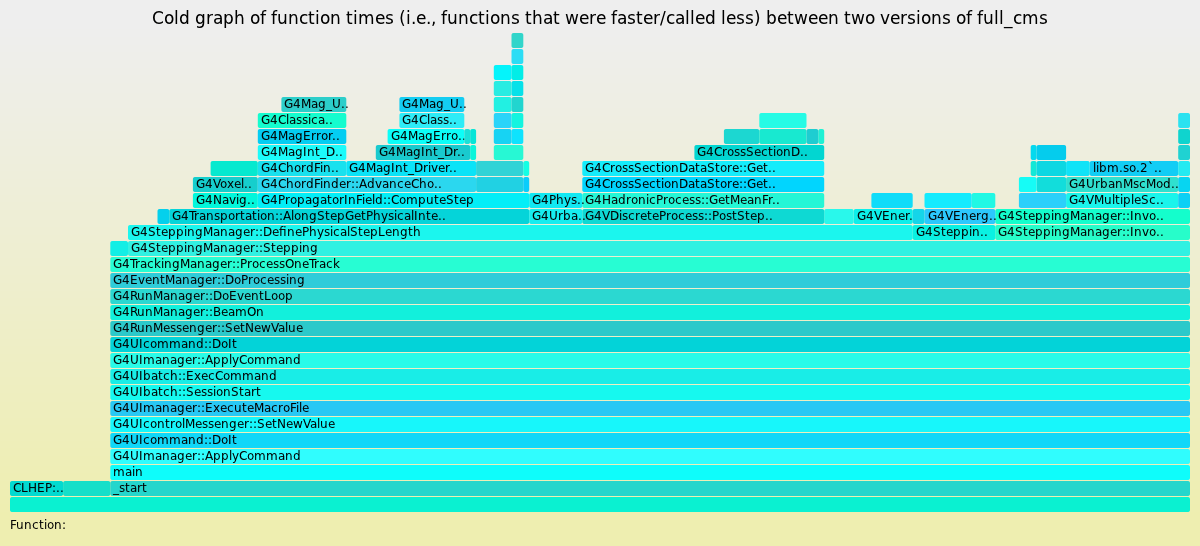
\includegraphics[width=1.0\textwidth]{dec.png}
\end{center}
\end{frame}

%%%%%%%%%%%%%%%%%%%%%%%%%%%%%%%%%%%%%%%%%%%%%%%%%%%%%%%%%%%%%%%%%%%%%%%%%%%%%%%%
%								PART 2
%%%%%%%%%%%%%%%%%%%%%%%%%%%%%%%%%%%%%%%%%%%%%%%%%%%%%%%%%%%%%%%%%%%%%%%%%%%%%%%%
\begin{frame}
\begin{center}
\fcolorbox{red}{white}{\huge{{\bf PART TWO}}}
\end{center}
\end{frame}

%%%%%%%%%%%%%%%%%%%%%%%%%%%%%%%%%%%%%%%%%%%%%%%%%%%%%%%%%%%%%%%%%%%%%%%%%%%%%%%%
%%%%%%%%%%%%%%%%%%%%%%%%%%%%%%%%%%%%%%%%%%%%%%%%%%%%%%%%%%%%%%%%%%%%%%%%%%%%%%%%
\begin{frame}{Overview}

\textcolor{blue}{Ideas explored}
\begin{itemize}
  \item {\bf Particle bunching (G4SmartTrackStack) }
  \item Hard-coded stepping manager (G4SteppingManager)
  \item Caching of cross-sections calculations in hadronic processes (G4CrossSectionDataStore)
  \item Reducing branch mispredictions in Value() (G4PhysicsVector)
  \item Caching values of ln(Energy) (G4Track)
\end{itemize}
\end{frame}

%%%%%%%%%%%%%%%%%%%%%%%%%%%%%%%%%%%%%%%%%%%%%%%%%%%%%%%%%%%%%%%%%%%%%%%%%%%%%%%%
%%%%%%%%%%%%%%%%%%%%%%%%%%%%%%%%%%%%%%%%%%%%%%%%%%%%%%%%%%%%%%%%%%%%%%%%%%%%%%%%
\begin{frame}{Particle "bunching"}
\textcolor{blue}{Definition}
Process \textit{same} particle types before switching to another particle type. E.g.,

\begin{equation*}
\ldots, e^-, e^-, \ldots, e^-, \gamma, \gamma, \ldots, \gamma, \ldots
\end{equation*}

\textcolor{blue}{Why} Better \textit{cache utilisation} due to access to the
same physics list

\vspace{5 mm}

Number of stacks we are using: 5

\begin{enumerate}
\item Primary particles + everything not belonging to:
\item Neutrons
\item Electrons
\item Gammas
\item Positrons
\end{enumerate}
\end{frame}

%%%%%%%%%%%%%%%%%%%%%%%%%%%%%%%%%%%%%%%%%%%%%%%%%%%%%%%%%%%%%%%%%%%%%%%%%%%%%%%%
%%%%%%%%%%%%%%%%%%%%%%%%%%%%%%%%%%%%%%%%%%%%%%%%%%%%%%%%%%%%%%%%%%%%%%%%%%%%%%%%
\begin{frame}{Particle "bunching" - Problems}

\textcolor{blue}{Problems}
\begin{itemize}
\item {\bf Stacks can grow very large}
\begin{itemize}
\item e.g., when processing electrons, the gamma stack explodes, and vice versa
\end{itemize}
\item Therefore, we have to {\bf restrict} them, which leads to another problem:
\begin{itemize}
\item What is the optimal size for each one?
\item How much aggressively should we process a track, once it has hit its upper limit ?
\end{itemize}
\end{itemize}
\end{frame}

%%%%%%%%%%%%%%%%%%%%%%%%%%%%%%%%%%%%%%%%%%%%%%%%%%%%%%%%%%%%%%%%%%%%%%%%%%%%%%%%
%%%%%%%%%%%%%%%%%%%%%%%%%%%%%%%%%%%%%%%%%%%%%%%%%%%%%%%%%%%%%%%%%%%%%%%%%%%%%%%%
\begin{frame}{Particle "bunching" - Problems cont.}
If we allow {\bf too large} stack sizes
\begin{itemize}
\item we diverge a lot in terms of geometry (it hurts)
\end{itemize}
If we allow {\bf too small} stack sizes
\begin{itemize}
\item we switch too often between stacks, and we thrash (it hurts)
\end{itemize}
\vspace{5mm}
If we are {\bf too aggressive} when penalizing the offending stack,
\begin{itemize}
\item by consuming its elements, then the other stacks will get inflated (it hurts)
\end{itemize}

\begin{center}
\fcolorbox{red}{white}{Outcome very dependent on the selection of above parameters}
\end{center}
\end{frame}

%%%%%%%%%%%%%%%%%%%%%%%%%%%%%%%%%%%%%%%%%%%%%%%%%%%%%%%%%%%%%%%%%%%%%%%%%%%%%%%%
%%%%%%%%%%%%%%%%%%%%%%%%%%%%%%%%%%%%%%%%%%%%%%%%%%%%%%%%%%%%%%%%%%%%%%%%%%%%%%%%
\begin{frame}{G4SmartTrackStack - Current state of things}
\textcolor{blue}{Current state}
The algorithm, in its current incarnation, does {\bf not} provide any benefit in
terms of performance.

\vspace{5mm}

\textcolor{blue}{Problems}
\begin{itemize}
\item Suboptimal choice of max stack sizes
\item Although G4SmartTrackStack tries to impose limits on the maximum size a
stack can grow to, there is a {\bf degenerate} case where it doesn't.
\end{itemize}
\end{frame}

%%%%%%%%%%%%%%%%%%%%%%%%%%%%%%%%%%%%%%%%%%%%%%%%%%%%%%%%%%%%%%%%%%%%%%%%%%%%%%%%
%%%%%%%%%%%%%%%%%%%%%%%%%%%%%%%%%%%%%%%%%%%%%%%%%%%%%%%%%%%%%%%%%%%%%%%%%%%%%%%%
\begin{frame}{G4SmartTrackStack - Modifications}

\textcolor{blue}{{\bf Reduce size of stacks}}
\begin{itemize}
\item ~5\% gain in 200 events, ~3\% in 1k events, ~1\% in 2k events, cross-over at 3k events
\end{itemize}
\textcolor{blue}{Impose {\bf hard limits} on the size of the stacks}
\begin{itemize}
\item First version ever to confer a {\bf persistent} reduction in total execution time, albeit small ($<1\%$)
\end{itemize}
\textcolor{blue}{Show {\bf affinity for low energy $e^-$} (+ hard limits)}
\begin{itemize}
\item Best version of particle bunching: 4-5\% {\bf persistent} reduction in total execution time
in FullCMS experiment (less in SimplifiedCalorimeter)
\end{itemize}
\end{frame}

%%%%%%%%%%%%%%%%%%%%%%%%%%%%%%%%%%%%%%%%%%%%%%%%%%%%%%%%%%%%%%%%%%%%%%%%%%%%%%%%
%%%%%%%%%%%%%%%%%%%%%%%%%%%%%%%%%%%%%%%%%%%%%%%%%%%%%%%%%%%%%%%%%%%%%%%%%%%%%%%%
\begin{frame}{G4SmartTrackStack}

\begin{center}
  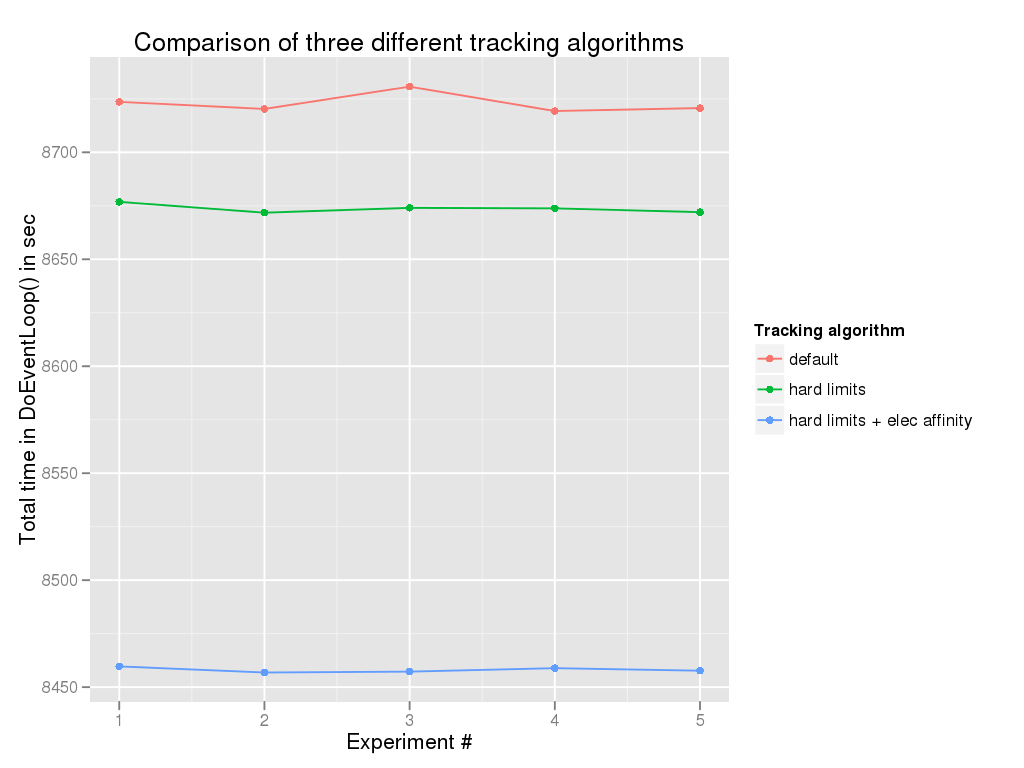
\includegraphics[width=1.0\textwidth]{trackingcmp.png}
\end{center}
\end{frame}

%%%%%%%%%%%%%%%%%%%%%%%%%%%%%%%%%%%%%%%%%%%%%%%%%%%%%%%%%%%%%%%%%%%%%%%%%%%%%%%%
%%%%%%%%%%%%%%%%%%%%%%%%%%%%%%%%%%%%%%%%%%%%%%%%%%%%%%%%%%%%%%%%%%%%%%%%%%%%%%%%
\begin{frame}[fragile]{Reducing branch mispredictions in Value G4PhysicsVector}

\textcolor{blue}{Objective} Calculate the cache hits ratio in G4PhysicsVector::Value()

\lstset{basicstyle=\tiny\ttfamily}
\lstset{frame=single, columns=flexible}
\begin{lstlisting}
# dtrace -qn '
/* 0xc0 is the offset inside Value() where a cache hit takes place */
pid$target::_ZN15G4PhysicsVector5ValueEd:c0
{ 
    @branch = count();
}

pid$target::_ZN15G4PhysicsVector5ValueEd:entry
{
    @total = count();
}

tick-100ms
{
    printa(@branch);
    printa(@total);
}' -c '/home/stathis/geant4.9.5.p01/bin/full_cms ./bench1_5k.g4' -o val
\end{lstlisting}
\end{frame}

%%%%%%%%%%%%%%%%%%%%%%%%%%%%%%%%%%%%%%%%%%%%%%%%%%%%%%%%%%%%%%%%%%%%%%%%%%%%%%%%
%%%%%%%%%%%%%%%%%%%%%%%%%%%%%%%%%%%%%%%%%%%%%%%%%%%%%%%%%%%%%%%%%%%%%%%%%%%%%%%%

\begin{frame}{Reducing branch mispredictions in Value G4PhysicsVector}
\begin{center}
  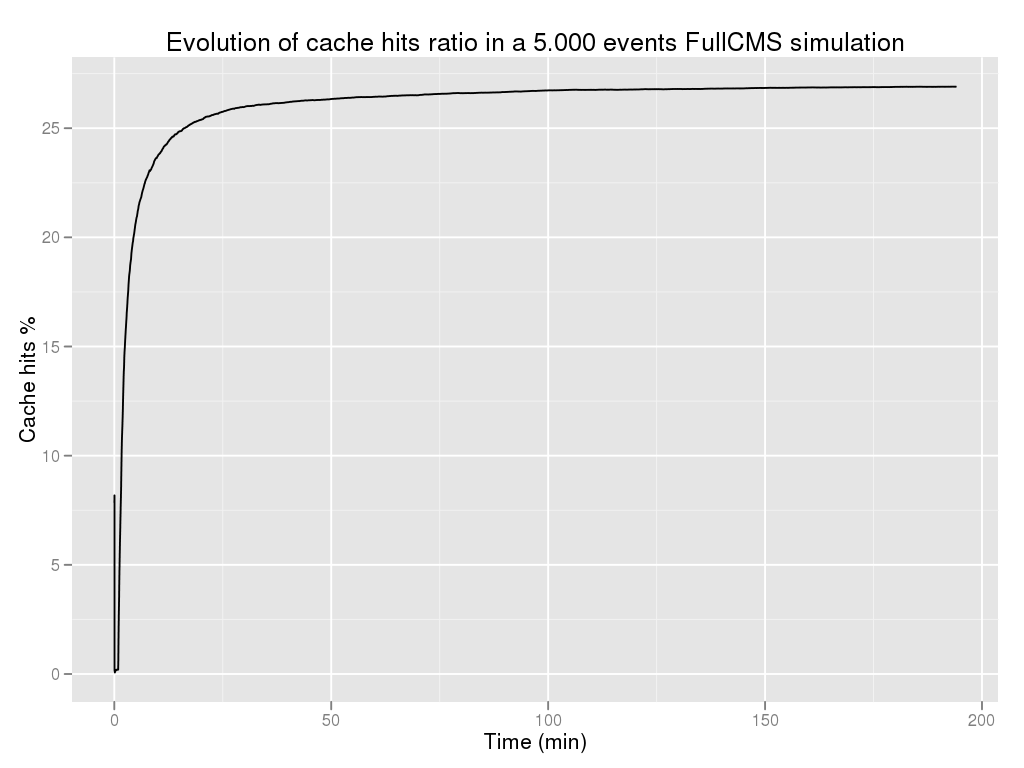
\includegraphics[width=1.0\textwidth]{G4PhysicsVector-Value.png}
\end{center}
\end{frame}

%%%%%%%%%%%%%%%%%%%%%%%%%%%%%%%%%%%%%%%%%%%%%%%%%%%%%%%%%%%%%%%%%%%%%%%%%%%%%%%%
%%%%%%%%%%%%%%%%%%%%%%%%%%%%%%%%%%%%%%%%%%%%%%%%%%%%%%%%%%%%%%%%%%%%%%%%%%%%%%%%

\begin{frame}{Reducing branch mispredictions in Value G4PhysicsVector}
\begin{itemize}
\item The cache hits ratio is not extraordinarily high,
\item ... yet the benefit of caching outweighs (as reality dictates) the penalty of
branch mispredictions
\item The eventual ratio is higher than that I had in mind initially
\item Lesson learnt: let the system reach its equilibrium before drawing any conclusions
\end{itemize}
\end{frame}

%%%%%%%%%%%%%%%%%%%%%%%%%%%%%%%%%%%%%%%%%%%%%%%%%%%%%%%%%%%%%%%%%%%%%%%%%%%%%%%%
%%%%%%%%%%%%%%%%%%%%%%%%%%%%%%%%%%%%%%%%%%%%%%%%%%%%%%%%%%%%%%%%%%%%%%%%%%%%%%%%
\begin{frame}

\textcolor{blue}{"Problem"} A flamegraph showing branch mispredictions identified
G4PhysicsVector::Value() as a significant offender

\vspace{5mm}

\textcolor{green}{Idea} Try to collapse some of the if-blocks, gaining branch
predictability, but executing more cpu instructions

\vspace{5mm}

\textcolor{red}{Result} The branch mispredictions reduced (expected), but the
the average time spent in that function was actually larger

\end{frame}

%%%%%%%%%%%%%%%%%%%%%%%%%%%%%%%%%%%%%%%%%%%%%%%%%%%%%%%%%%%%%%%%%%%%%%%%%%%%%%%%
%%%%%%%%%%%%%%%%%%%%%%%%%%%%%%%%%%%%%%%%%%%%%%%%%%%%%%%%%%%%%%%%%%%%%%%%%%%%%%%%
\begin{frame}{DTrace - Introduction 1/2}
\begin{itemize}
\item ``D'' stands for Dynamic- it dynamically instruments a running program,
by modifying its instructions while it is executing
\item {\bf Deep inspection}
\begin{itemize}
\item Arbitrary instructions
\item CPU registers
\item CPU hardware counters, etc
\end{itemize}
\item {\bf Sophisticated profiling} (e.g., speculative tracing)
\vspace{5mm}
\item {\bf Built-in aggregation} functions
\begin{itemize}
\item count, sum, avg, min, max, stddev, \{l,\}quantize
\end{itemize}

\item {\bf Negligible runtime overhead}
\end{itemize}
\end{frame}

\begin{frame}{DTrace - Introduction 2/2}
\begin{itemize}
\item {\bf Safe} to use in production environments
\begin{itemize}
\item Safety was one of the central architectural decisions upon DTrace was built
\item Explains why some common language constructs aren't supported (e.g., for-loops)
\end{itemize}

\item {\bf No source code modification} of the profiled application needed
\item Can operate on {\bf multithreaded} programs (has support for thread-local variables)
\item Runs on {\bf Mac OSX} out of the box; Linux port is on the way
\item Profiling done via a simple language called D (resembling C and awk)
\begin{itemize}
\item Scripts can be shared, reviewed, reused, made be run unattended
\end{itemize}
\end{itemize}
\end{frame}

%%%%%%%%%%%%%%%%%%%%%%%%%%%%%%%%%%%%%%%%%%%%%%%%%%%%%%%%%%%%%%%%%%%%%%%%%%%%%%%%
%%%%%%%%%%%%%%%%%%%%%%%%%%%%%%%%%%%%%%%%%%%%%%%%%%%%%%%%%%%%%%%%%%%%%%%%%%%%%%%%
\begin{frame}{Future plans}

\begin{itemize}
\item Document everything- positive and negative results
\item Break up commits so that each one introduces only one feature
\item Try to reproduce the results in a computing environment closer to CERN's
\end{itemize}
\end{frame}

%%%%%%%%%%%%%%%%%%%%%%%%%%%%%%%%%%%%%%%%%%%%%%%%%%%%%%%%%%%%%%%%%%%%%%%%%%%%%%%%
%%%%%%%%%%%%%%%%%%%%%%%%%%%%%%%%%%%%%%%%%%%%%%%%%%%%%%%%%%%%%%%%%%%%%%%%%%%%%%%%
\def\UrlFont{\scriptsize\ttfamily}
\begin{frame}{Documentation}

\textcolor{blue}{Documentation will be appearing in the following links:}

\begin{itemize}
\item \url{http://leaf.dragonflybsd.org/~beket/geant4/dtrace.html}
\item \url{http://leaf.dragonflybsd.org/~beket/geant4/solaris.html}
\end{itemize}

\vspace{5mm}

\begin{itemize}
\item \url{http://island.quantumachine.net/~stathis/geant4/smartstack.html}
\item \url{http://island.quantumachine.net/~stathis/geant4/crosssections.html}
\item \url{http://island.quantumachine.net/~stathis/geant4/hardstepping.html}
\item \url{http://island.quantumachine.net/~stathis/geant4/lnenergy.html}
\end{itemize}
\end{frame}

%%%%%%%%%%%%%%%%%%%%%%%%%%%%%%%%%%%%%%%%%%%%%%%%%%%%%%%%%%%%%%%%%%%%%%%%%%%%%%%%
%%%%%%%%%%%%%%%%%%%%%%%%%%%%%%%%%%%%%%%%%%%%%%%%%%%%%%%%%%%%%%%%%%%%%%%%%%%%%%%%
\begin{frame}{The end}
\vspace*{\fill}
\begin{center}
Thank you. Questions?
\end{center}
\vspace*{\fill}
\end{frame}

\end{document}
